%نام و نام خانوادگی:
%شماره دانشجویی: 
\مسئله{ }

\پاسخ{



 ابتذا می‌آییم کد tac مربوط به آنرا مینویسیم:
\lr{\lstinputlisting[]{commons/Q2.java}}
\begin{figure}[H]
			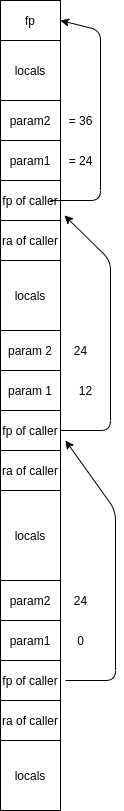
\includegraphics[width=\linewidth]{./commons/Q2.png}
			\label{fig:Q2}
		\end{figure}  
		
	اولین بار که خط یازده اجرا میشود با توجه به استک فریم در 16 * 4 تا پایین تر کال میشود  و مسوول pushکردن آن پارامتر ها تابع gcdای است که اولین بار کال مبشود.
	اولین بار که خط هشت کال میشود fp در 25 * 4 تا پایین تر است و مسوول ;صدا کردن این تابع gcd ای است که قبل از آن کال شده است و مقدار را به تابع بالاتر میدهد و پاپ پارامز را انجام میدهد.
}

